\documentclass{ximera}
\usepackage{tikz}
\author{Jeffrey Kuan}
\input{../preamble} %% Loads the graphics path
\title{Introduction to Quantum Groups and Yang-Baxter Equation For Probabilists}
\license{CC: 0}
\begin{document}

\begin{abstract}
   The Yang--Baxter equation is cool. 
\end{abstract}
\maketitle
%\part{Introduction}
%\chapterstyle
%    \activity{basics/basicWorksheet}
%    \sectionstyle
%    \activity{basics/exercises/someExercises}

%    \chapterstyle
%    \activity{basics/graphicsInteractives}

Accessibility statement: these notes will eventually be WCAG2.1AA compliant, once I finish writing them. I tested it out using NVDA, a screen reader.
It works best if you uncheck ``graphic'' and ``clickable'' in the settings. 


\section{Introduction}

Broadly speaking, \textbf{integrable probability} is a branch of probability theory which studies 
models which have exact solutions. For this reason, these models are often called \textbf{exactly solvable.}
From these exact solutions, one can derive precise \textbf{universal} asymptotics, such as the 
famed Tracy--Widom distribution. The origin of these solutions are usually due to algebraic symmetries 
underlying the model. In these set of lecture notes, we will introduce the relevant algebraic background
with a probabilistic researcher as the target audience. 

For historical context, the terminology originates in integrable systems from Hamiltonian mechanics.
In Hamiltonian mechanics, the phase space is represented as a smooth manifold with even dimension $2n,$
with coordinates denoted $q_1,\ldots,q_n,p_1,\ldots,p_n$ for the momentumm and position. An integrable
system is a system with $n$ conserved quantities, and the Liouville--Arnold theorem states that the 
equations of motion can be solved in quadratures. For an explicit example, the harmonic oscillator in 
one dimension (imagine an object attached to a frictionless spring) is integrable, and the conserved quantity
is the total energy. In contrast, the three--body problem is not integrable, and its solutions are 
notoriously non--exact. 

During the 1980s, many Soviet mathematicians and physicsts introduced quantum mechanics into integrable
systems. In quantum mechanics, quantities such as position, momentum and energy became operators which 
generally do not commute; additionally, the values of these quantities only take discrete, ``quantized''
values. In this context, the concept of ``conserved quantities'' becomes ``commuting operators,'' and 
values of the quantities are eigenvalues of eigenstates. At the time, their approaches were called the
``quantum inverse scattering method.'' Since then, the method has been generalized to abstract 
algebraic objects, such as Hopf algebras. 

These notes will introduce one such algebraic object, known as \textbf{quantum groups,} with a particular
focus on the Yang--Baxter equation. The exposition will use probability and mathematical physics as a
motivation. The goal is for a reader with a probability background to be able to read contemporary (as of
2024) research papers in integrable probability. 

\textbf{Acknowledgements.} The author was supported by the London Mathematical Society. 

\section{ASEP, XXZ, and $U_q(sl_2)$}

To begin to motivate the notes, we first introduce the asymmetric simple exclusion process (ASEP) and its relationship to 
the Heisenberg XXZ model and the quantum group $U_q(sl_2).$ 

\subsection{Definition of ASEP}
In ASEP, particles randomly jump on a lattice, which we assume to be
one--dimensional. At most one particle may occupy a site, and jumps to occupied sites are blocked (hence the term ``exclusion'').
Jumps are nearest neighbour (hence the term ``simple''). If the jumps are continuous--time exponential 
clocks with left rates $\alpha$ and right rates $\beta,$ then let $q=\sqrt{\beta/\alpha}$ denote the 
asymmetry parameter. If $q\neq 1,$ then the model is asymmetric (sometimes partially asymmetric), 
while for $q=1$ the model is symmetric. For $q=0$ or $q=\infty$ the model is called totally asymmetric.
The symmetric exclusion process (without the word simple) can be defined more generally on an arbritrary graph. In princple, so can 
the asymmetric exclusion process, although this is not as well studied.  

\includegraphics{ASEPScreenshot.png}

The generator of the simple exclusion process can be explicitly written. In the most elementary case 
where there are two lattice sites, then there are four possible configurations. Associate to each
particle the vector $[1\ 0]$ and to each hole (i.e. a non--particle) the vector $[0 \ 1].$ Tensoring
the vectors together, we can associate to each configuration a canonical basis element of the four--dimensional
vector space $\mathbb{C}\otimes \mathbb{C}.$ The field here is chosen to be the complex numbers because
it is algebraically closed, although of course probabilities are real numbers. 

\includegraphics[height=0.3cm]{ASEPConfigurations.png}

With that set up, the generator is then a $4\times 4$ matrix
$$
\alpha\left(
    \begin{array}{cccc}
       0 & 0 & 0 & 0 \\
       0 & -1 & 1 & 0 \\
       0 & q^2 & -q^2 & 0 \\
       0 & 0 & 0 & 0 
    \end{array}
\right).
$$
The constant $\alpha$ can be viewed as a time rescaling, so it can be removed without loss of generality. 

In a more general setting, where there are $N$ lattice sites, the generator can be defined from the
above \(4\times 4\) matrix, which we now denote \(\mathcal{L}.\) The generator is now a \(2^N \otimes 2^N\) and
acts on  \((\mathbb{C}^2)^{\otimes N}.\) Define \(\mathcal{L}_{i,i+1}\) by 
\[
\mathcal{L}_{i,i+1} = (\mathrm{Id}_2)^{i-1} \otimes \mathcal{L} \otimes (\mathrm{Id}_2)^{N-1}.
\]
With this notation, the generator is
\[
\sum_{i=1}^{N-1} \mathcal{L}_{i,i+1}.
\]
Similar notation using subscripts will be used throughout these notes.

\subsection{ASEP and Yang--Baxter Equation}
The corresponding notion of integrability in the quantum case comes from Yang--Baxter equation. 
It was shown by Baxter that when a matrix solves the Yang--Baxter equation, there are corresponding
``commuting transfer matrices,'' which are analogous to conserved quantities in the classical setting. 



Using the same notation as in the previous section, 
we say that a matrix \(R\) solves the \underline{braided Yang--Baxter Equation} if:
\[
R_{12}R_{23}R_{12} = R_{23}R_{12}R_{23}.
\]
Somewhat confusingly, this equation is also sometimes called the braid equation or just the Yang--Baxter equation.
An equivalent formulation is
\[
R_{12}R_{13}R_{23} = R_{23}R_{13}R_{12}
\]
(exercise left to the reader). 

A visual representation of YBE is given by this image:

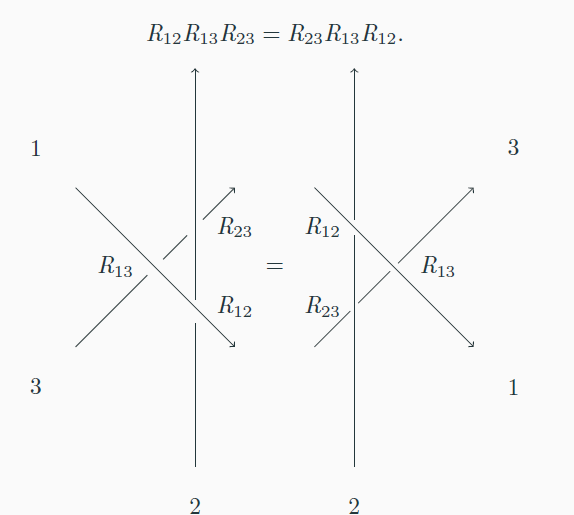
\includegraphics[height=8cm]{YBEScreenshot.png}

In some settings, the YBE occurs in the scattering of particles with quantum mechanics considerations, 
such as the QISM (quantum inverse scattering method.)

Given an arbitrary matrix \(R,\) one can check that it satisfies the YBE
through direct computation. However, it maybe more helpful to consider some simple examples first. 

If \(P: V \otimes V \rightarrow V \otimes V\) denotes the permutation operator which sends
\(u \otimes v\) to \(v \otimes u,\) then the braided Yang--Baxter equation becomes an identity of transpositions:
\[
(1\ 2) \circ (2 \ 3 ) \circ (1 \ 2 ) = (2 \ 3) \circ (1 \ 2) \circ (2 \ 3).
\]
This identity holds, since both sides equal the permutation \((1\ 3).\) An even more simple solution is 
the identity matrix. 

A probabilist may remark that a permutation matrix and an identity matrix are both examples of a stochastic matrix,
albeit somewhat trivial examples. It may then be natural to try to find more general stochastic matrices
which solve the Yang--Baxter equation. The ``simplest'' generalization occurs when \(V\) is two--dimensional,
with basis \(e_1,e_2.\) Using exclusion processes as a prototype, we can define the operator $R_{\alpha\beta}$
by
\[
R_{\alpha\beta}(e_1 \otimes e_1) = e_1 \otimes e_1, \quad R_{\alpha\beta}(e_2\otimes e_2) = e_2 \otimes e_2
\]
and
\begin{align*}
R_{\alpha\beta}(e_1 \otimes e_2) &= (1-\alpha)e_1 \otimes e_2 + \alpha e_2 \otimes e_1,\\
R_{\alpha\beta}(e_2 \otimes e_1) &= \beta e_1\otimes e_2 + (1-\beta)e_2 \otimes e_1.
\end{align*}
Inserting this matrix into the Yang--Baxter equation and evaluating at \(e_1 \otimes e_1 \otimes e_2,\)
one finds that \(\alpha(1-\beta)=0\) is a necessary requirement for a solution to YBE. Evaluating
\( R_{\alpha,1}\) and \(R_{0,\beta}\) at \(e_1\otimes e_2 \otimes e_1\) and \(e_2 \otimes e_1 \otimes e_1\)
yields no aditional equations. (Exercise left to the reader)

One could also evaluate YBE at the three vectors \(e_2 \otimes e_1 \otimes e_1,e_1\otimes e_2 \otimes e_1\)
and \(e_1 \otimes e_1 \otimes e_2,\) but instead we use another symmetry of ASEP. This is called
\underline{particle--hole involution.} In words, in an ASEP with drift to the right, the holes evolve
as an ASEP with drift to the left. Symbolically, we define an involution \(T\) of \(V\) which
switches \(e_1\) and \(e_2.\) Then 
\[
T^{\otimes 2} R_{\alpha,\beta}T^{\otimes 2} = R_{\beta,\alpha}, \quad \quad T^{\otimes 2} R_{\alpha,\beta} = R_{1-\alpha,1-\beta}, \quad \quad R_{\alpha,\beta}T^{\otimes 2} = R_{1-\beta,1-\alpha}.
\]
A mildly helpful observation here is that \(T\) is stochastic, so its composition with other stochastic
matrices is also stochastic. Using these identities, one immediately verifies YBE for 
\(R_{\alpha,0}\) and \(R_{1,\beta}.\) Furthermore, these two solutions are related up to the particle--hole involution.

One notices that \(R_{\alpha,0}-\mathrm{id}_4\) is the generator of ASEP at two lattice sites. It is then
natural to ask whether or not addition by constants affects integrability. The answer is ``no'' (otherwise 
integrable probability would not exist). As some intuition, let us suppose that the generator has an 
explicit set of eigenvectors and eigenvalues. In general, an arbitrary Markov process will have 
complicated eigenvectors and eigenvalues, but for integrable models we expect ``nice'' eigenvectors
and eigenvalues, from which probabilistic information can be extracted. Then addition by constants leaves
the eigenvectors unaffects and only shifts the eigenvalues, leaving them just as ``nice.'' Thus, 
it is fair to say that ASEP is integrable, at least on two lattice sites. 

At this juncture, it is reasonable to object that nothing has been said about the integrability of ASEP
on arbitrarily many lattice sites. We will put this question on hold, as the next section's discussion
of the XXZ model will lay the foundation for answering this question.


\subsection{XXZ model}
Having established that ASEP is an integrable model at two lattice sites, it is natural to ask about
other integrable models that look similar to ASEP, so that we can avoid re--inventing the wheel. Thus we 
now turn our attention to a related model, called the quantum Heisenberg model. These were introduced
by Werner Heisenberg to incorporate quantum mechanics into magnetism. Each lattice site has a microscopic
magnetic dipole, which can either be up or down. If there are \(N\) lattice sites, 
then the Hamiltonian acts on the \(2^N\)--dimensional vector space \((\mathbb{C}^2)^{\otimes N}.\)
So, at the very least, the state space of the XXZ model is the same as the ASEP state space. 

To define the model, first recall that Pauli spin matrices:
\[
\sigma^1 = \left(\begin{array}{cc} 0 & 1 \\ 1 & 0 \end{array}\right), \quad \quad \sigma^2 = \left( \begin{array}{cc} 0 & -i \\ i & 0 \end{array}\right), \quad \quad \sigma^3 = \left( \begin{array}{cc} 1 & 0 \\ 0 & -1 \end{array}\right).
\]
The notation \(\sigma^x,\sigma^y,\sigma^z\) are often used instead. 
Note that these are traceless and are Hermitian, the latter property being important in physics (since
Hermitian matrices have real eigenvalues, and these eigenvalues correspond to physical quantities). 
Letting
\[
\sigma^a_j = (\mathrm{Id})^{\otimes j-1} \otimes \sigma^a \otimes (\mathrm{Id})^{\otimes N-j}
\] 
so that \(\sigma^a_j\) acts on the \(j\)--th lattice site while fixing the others, the Hamiltonian is then
\[
\frac{-1}{2}\sum_{j=1}^N \left( J_x \sigma^1_j \sigma^1_{j+1} + J_y \sigma^2_j \sigma^2_{j+1} + J_z \sigma^3_j\sigma^3_{j+1} - h\sigma^3_j\right).
\]
where \(J_x,J_y,J_z\) are some coupling constants and \(h\) is the external field. We impose periodic boundary
conditions, so that \(\sigma^a_{N+1}=\sigma^a_1.\) If \(J_x,J_y,J_z\) are distinct then one obtains the 
XYZ model. If \(J_x=J_y \neq J_z\) then this is the XXZ model; if \(J_x=J_y=J_z\) then it is the XXX model.

Each summand in the Hamiltonian can be written as a four by four matrix:
\[
\left(\begin{array}{cccc}
J_z + 2h & 0 & 0 & J_x-J_y \\
0 & -J_z & J_x + J_y & 0 \\
0 & J_x + J_y & -J_z & 0 \\
J_x - J_y & 0 & 0 & J_z-2h
\end{array}\right)
\]
If \(J_x=J_y,\) as assumed in the XXZ model, then the top--right and bottom--left entries are zero. In 
this case, the non--zero entries are at least the same as in the ASEP generator. Recalling the previous
section's heuristic that adding by constants does not change integrability, we can set \(J_z=1,h=0\) to
obtain the matrix
\[
\mathrm{Id}_4 + \left( \begin{array}{cccc}
0 & 0 & 0 & 0 \\
0 & -2 & 2J_x & 0 \\
0 & 2J_x & -2 & 0\\
0 & 0 & 0 & 0 
\end{array}\right).
\]

At this point, it is worth noticing that the YBE is a statement about operators on vector spaces, 
which should not depend on the choice of bases on the vector spaces. In other words, conjugation 
(which corresponds to a change of basis) should not affect integrability. As it turns out, conjugation by 
\[
\left( \begin{array}{cccc}
1 & 0 & 0 & 0 \\
0 & 1 & \gamma-1 & 0 \\
0 & 0 & \gamma & 0 \\
0 & 0 & 0 & 1
\end{array} \right)
\]
results in the ASEP generator on two sites. (Exercise left to the reader).



\subsection{\(sl_2\) symmetry}
So far, we have determined that ASEP is integrable and is conjugate to the XXZ Hamiltonian
(assuming that we are ignoring the question of arbitrary lattice sizes). As it turns out, the
Pauli matrices form a basis of the real Lie algebra \(su_2\) corresponding to the real compact Lie group 
\(SU(2).\) Here, a real Lie group means that the underlying field is the real numbers, not that
all the entries are real (consider the unit circle in the complex plane as a real Lie group, for example).

The complex variant of \(SU(2)\) is the (non--compact) Lie group \(SL(2,\mathbb{C})\) of traceless 
\(2 \times 2\) matrices with complex entries. For a variety of reasons, some of which answer historical,
most mathematicians are introduce to the Lie algebra \(sl_2\) rather than \(su_2,\) so we will use that notation.

By definition, \(sl_2\) is the Lie algebra with basis denoted \(e,f,h\) and brackets
\[
[e,f]=h, \quad [h,e]=2e, \quad [h,f]=-2f.
\]
Note that the explicit matrices \(E_{12},E_{21},E_{11}-E_{22}\) satisfy these relations, where
\(E_{ij}\) denotes the matrix with a \(1\) at the \(i,j\)--entry and a 0 everywhere else. 

Returning to the XYZ model, one can calculate that the XXX model has \(SU(2)\) symmetry (exercise to the
reader) in the sense that
\[
\sum_{j=1}^N \sigma^a_j
\]
commutes with the Hamiltonian of the XXX model for \(a=x,y,z.\) However, for the XXZ model, the
commutation only works for \(a=z.\) Therefore, whatever algebra is underlying the XXZ model (and hence
that of ASEP), we know that it can not be as simple as \(SU(2).\) Futhermore, since XXZ and ASEP have
a free parameter, the algebra should be a one--parameter deformation of \(SU(2).\) This leads into
the next topic of quantum groups. 

\section{Quantum Group \(U_q(sl_2)\)}
The Drinfel'd--Jimbo quantum groups are quantizations of the Lie groups. Rather confusingly, the
quantum groups are not themselves groups. 

Before diving into the rigorous definition, one notes where the quantization occurs. Using probabilistic
intuition, we expect that the SSEP should have an underlying \(sl_2\) symmetry, whereas the
ASEP should have the quantum group symmetry. However, SSEP and ASEP on a single lattice site are
identical, so the quantization must require multiple lattice sites. We've established that in this
case, the vector space is \((\mathbb{C}^{\otimes 2})^{\otimes N}.\) This raises the question:
how does \(sl_2\) act on tensor powers?

To answer this question, we take an aside about Lie algebras, which are tangent spaces to Lie groups
at the origin. What this implies is that for a Lie group \(G\) with a Lie algebra \(g,\) we have that
\[
X \in g \text{ implies } \exp(tX) \in G \text{ for all } t\in \mathbb{R}
\]
and
\[
X = \frac{d}{dt} \exp(tX) \Big|_{t=0}.
\]
Setting \(g=g_X(t)=\exp(tX),\) the natural action of a group on tensor products is
\[
g(v \otimes w)= gv \otimes gw.
\]
Taking derivatives and heuristically using Leibniz's rule for derivative of products, we obtain
\[
X(v \otimes w) = Xv \otimes w + v \otimes Xw.
\]
This is expressed through the \underline{co--product} \(\Delta: g \rightarrow g \otimes g\) defined by 
\[
\Delta(X) = 1 \otimes X + X \otimes 1.
\]

Since it is the co--product that allows for the algebra to act on multiple lattice sites (i.e. tensor powers),
the quantization occurs in the co--product, not the algebra itself! As it turns out, the right deformation is
\[
\Delta(e) = q^h \otimes e + e \otimes 1, \quad \Delta(f) = 1 \otimes f + f \otimes q^{-h}, \quad \Delta(h)=h\otimes 1 + 1\otimes h,
\]
where we interpret \(q^h\) as a formal power series in \(h.\) Note that we do not deform the co--product
of \(h,\) which is consistent with \(\sigma^z\) commuting with the XXZ model. 

Depending on the preferences of the author, the generator \(h\) may be replaced with \(k:=q^h\) with 
the co--product becoming
\[
\Delta(k) = k \otimes k.
\]
(Exercise to the reader why that is the same co--product). In words, \(h\) is primitive and \(k\) is 
group--like.

\subsection{Co-algebras and bi--algebras}
While I presented the co--product as the object that allows for multiple lattice sites, that is of 
course not how it is presented to algebraists. A more common description is that a co--algebra is
dual to an algebra, with the co--product dual to the product. This subsection will provide a rigorous
definition of a co--algebras.

Recall that an algebra \(A\) is a vector space with a multiplication operator
\[
m: A \otimes A \rightarrow A   
\]
which assumed to be bilinear. It is also associative in the sense that
\[
m(x \otimes m(y \otimes z)) = m(m(x \otimes y) \otimes z),   
\]
which essentially means that \( x(yz) = (xy)z.\) This is equivalently stated as
\[
m \circ (m \otimes \mathrm{id})   = m \circ (\mathrm{id} \otimes m).
\]
Additionally, there is an identity element \(1 \in A\) satisfying
\[
m(1 \otimes x) = m(x \otimes 1) = x.   
\]
This can be written as an inclusion from the underlying field \(F\) to the algebra \(A.\)

Before defining co--algebras, it will be useful to draw certain commutative diagrams. The associativity
can be written as
\begin{tikzpicture}
 \node (top) at (0,0) {\(A \otimes A \otimes A\)};
 \node (left) at (-5,-5) {\(A \otimes A\)};
 \node (right) at (5,-5) {\(A \otimes A\)};
 \node (bottom) at (0,-10) {\(A\)};
 \draw[black,-latex,line width=2pt] (top)--(left) node[midway,above] () {$m \otimes \mathrm{id}$};
 \draw[black,-latex,line width=2pt] (top)--(right) node[midway,above] () {$\mathrm{id} \otimes m$};
 \draw[black,-latex,line width=2pt] (left)--(bottom) node[midway,above] () {$m$};
\end{tikzpicture}





\section{Solutions to YBE, explicitly (less algebraic)}

RTT construction?

Fusion?

Orthogonal polynomial vertex weights?

\section{Research?}

\end{document}